\documentclass[12pt,twoside]{article} 
\usepackage{amsmath, amssymb} 
\usepackage{graphicx}
\usepackage{amsmath} 
\usepackage[active]{srcltx} 
\usepackage{amssymb} 
\usepackage{amscd} 
\usepackage{makeidx} 
\usepackage{amsthm} 
\usepackage{algpseudocode} 
\usepackage{algorithm}
\usepackage[spanish, activeacute]{babel}
\usepackage[utf8]{inputenc}

\renewcommand{\baselinestretch}{1}
\setcounter{page}{1}
\setlength{\textheight}{21.6cm}
\setlength{\textwidth}{14cm}
\setlength{\oddsidemargin}{1cm}
\setlength{\evensidemargin}{1cm}
\pagestyle{myheadings}
\thispagestyle{empty}
\markboth{\small{Pr\'actica 6. Fernando Rivera, Alejandro Contreras}}{\small{.}}

\begin{document}
\centerline{\bf An\'alisis de Algoritmos, Sem: 2020-1, 3CV2, Pr\'actica 6}
\centerline{}
\centerline{01 - 10 - 2019}
\begin{center}
\Large{\textsc{Pr\'actica 6: Máximo subarreglo}}
\end{center}
\centerline{}
\centerline{\bf {Rivera Paredes Fernando Daniel, Contreras Paredes Alejandro.}}
\centerline{}
\centerline{Escuela Superior de C\'omputo}
\centerline{Instituto Polit\'ecnico Nacional, M\'exico}
\centerline{$ferny036@hotmail.com, acontrerasparedes@hotmail.com$}
\newtheorem{Theorem}{\quad Theorem}[section] \newtheorem{Definition}[Theorem]{\quad Definition} \newtheorem{Corollary}[Theorem]{\quad Corollary} \newtheorem{Lemma}[Theorem]{\quad Lemma} \newtheorem{Example}[Theorem]{\quad Example} \bigskip
\textbf{Resumen:} Tomamos en cuenta un nuevo algoritmo, \textbf{Máximo Subarreglo} de un arreglo, la cual analizaremos de manera analítica y gráfica 
para dar a entender su comportamiento ante diversas situaciones, como puede ser su forma recursiva o por fuerza bruta
\centerline{}
{\bf Palabras Clave:} Máximo Subarreglo, Cuadrático, Divide y Vencerás, Lineal, Recursividad
\newpage

\section{Introducción}
El problema del su arreglo máximo es el método para encontrar el subarreglo continuo dentro de una matriz unidimensional de números que tiene la suma más grande.

El problema fue propuesto originalmente por Ulf Grenander de la Brown University en 1977, como un modelo simplificado para la estimación de máxima probabilidad de patrones en imágenes digitalizadas.

Podemos resolver este problema, consideremos una lista de varios enteros. Podríamos estar interesados ​​en cuál subconjunto completamente adyacente tendrá la mayor suma. Por ejemplo, si tenemos la matriz [0, 1, 2, -2, 3, 2] ,
el subarreglo máximo es [3, 2], con una suma de 5.
\newpage
\section{Conceptos B\'asicos} 
\subsection{\textbf{Máximo Subarreglo}}
\setlength{\parindent}{1.5em}El problema del máximo subarreglo consiste en encontrar un subarreglo, subarray o subvector de una determinada longitud $m$ cuya suma sea máxima dentro de un vector de longitud $n$, con $m \leq n$.
Este problema se puede resolver aplicando la técnica del algoritmo divide y vencerás, formando problemas cada vez más pequeños hasta alcanzar un caso base y posteriormente combinando las soluciones obtenidas. En concreto, la forma de aplicar el 
método algorítmico citado consiste en obtener los segmentos de suma máxima correspondientes a las mitades izquierda y derecha del vector y a la parte central para, una vez calculados, elegir el máximo de los tres. El algoritmo tiene un coste 
lineal respecto al tiempo.

\begin{figure}[h]
  \centering
    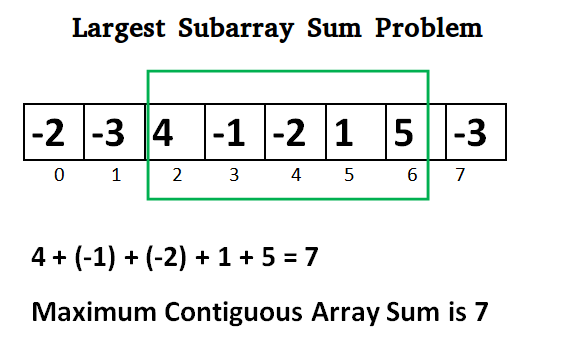
\includegraphics[height=0.5\textwidth]{Figure1}
  \caption{Máximo Subarreglo}
  \label{fig:ejemplo1}
\end{figure}

Para hacer incapie sobre el algoritmo de \textbf{Máximo Subarreglo} haremos uso de otro de forma lineal de manera que nos permita aplicar de nuevo la técnica de \textbf{Divide y Vencerás}, para reducir la complejidad en el mismo,
estamos hablando en si del algoritmo \textbf{Máximo Subarreglo Cruzado}.

\newpage
\section{Experimentaci\'on y Resultados}
\centerline{}
\subsection{\textbf{Máximo Subarreglo Cruzado}}
\begin{algorithm}
  \caption{Máximo Subarreglo Cruzado}\label{euclid}
  \begin{algorithmic}[1]
  \Function{MSC}{$A[0, ..., m-1], bajo, mitad, alto$}
      \State $suma \gets 0$                                             \Comment $O(1)$
      \State $n \gets alto - bajo + 1$                                  \Comment $O(1)$
      \State $suma\_izq \gets -\infty$                                  \Comment $O(1)$
      \State $max\_izq \gets suma\_izq$                                 \Comment $O(1)$
      \For{$i = mitad$ \textbf{to} $abajo$}                             \Comment $O(n)$
        \State $suma \gets suma + A[i]$                                 \Comment $O(1)$
        \If{$suma > suma\_izq$}                                         \Comment $O(1)$
          \State $suma\_izq \gets suma$                                 \Comment $O(1)$
          \State $max\_izq \gets i$                                     \Comment $O(1)$
        \EndIf                                                          
      \EndFor
      \State $suma \gets 0$                                             \Comment $O(1)$
      \State $suma\_der \gets 0$                                        \Comment $O(1)$
      \State $max\_der \gets suma\_der$                                 \Comment $O(1)$
      \For{$i = mitad + 1$ \textbf{to} $alto$}                          \Comment $O(n)$
        \State $suma \gets suma + A[i]$                                 \Comment $O(1)$
        \If{$suma > suma\_der$}                                         \Comment $O(1)$
          \State $suma\_der \gets suma$                                 \Comment $O(1)$
          \State $max\_der \gets i$                                     \Comment $O(1)$
        \EndIf                                                          
      \EndFor
      \State \textbf{return} $(max\_izq, max\_der, suma\_izq + suma\_der)$\Comment $O(1)$
  \EndFunction
  \end{algorithmic}
\end{algorithm}

La cual para verificar analíticamente su grado de complejidad de acuerdo a los comentarios, de una manera simplificada lo podemos ver de la siguiente
manera: 

\centerline{$T(n) = 8*O(1)+O(n)[4*O(1)]+O(n)[4*O(1)]$}
\centerline{}
\centerline{donde: $S = s(n)$}
\centerline{}
\centerline{donde: $O(g(n))_{1} + O(g(n))_{2}+\cdots+O(g(n))_n = O(g(n))$}
\centerline{}
\centerline{$\Rightarrow T(n) = O(1)+O(n)[O(1)]$}
\centerline{}
\centerline{donde: $O(f(n)) * O(g(n))= O(f(n)*g(n))$}
\centerline{}
\centerline{$\Rightarrow T(n) = O(1) + O(n)$}
\centerline{}
\centerline{donde: $O(f(n)) + O(g(n)) = O(h(n))$}
\centerline{y $h(n)$ es la funci\'on con mayor jeraqu\'ia respecto a $g(n)$ y $f(n)$}
\centerline{}
\centerline{$\therefore T(n) \in O(n) $}

Donde podemos notar que el algoritmo que utilizamos de ayuda tiene complejidad lineal $O(n)$, por tanto no genera una carga computacional
al momento de ejecutarla, de tal manera que procederemos a analizar ahora si nuestro algoritmo de \textbf{Máximo Subarreglo}.
\begin{figure}[h]
  \centering
    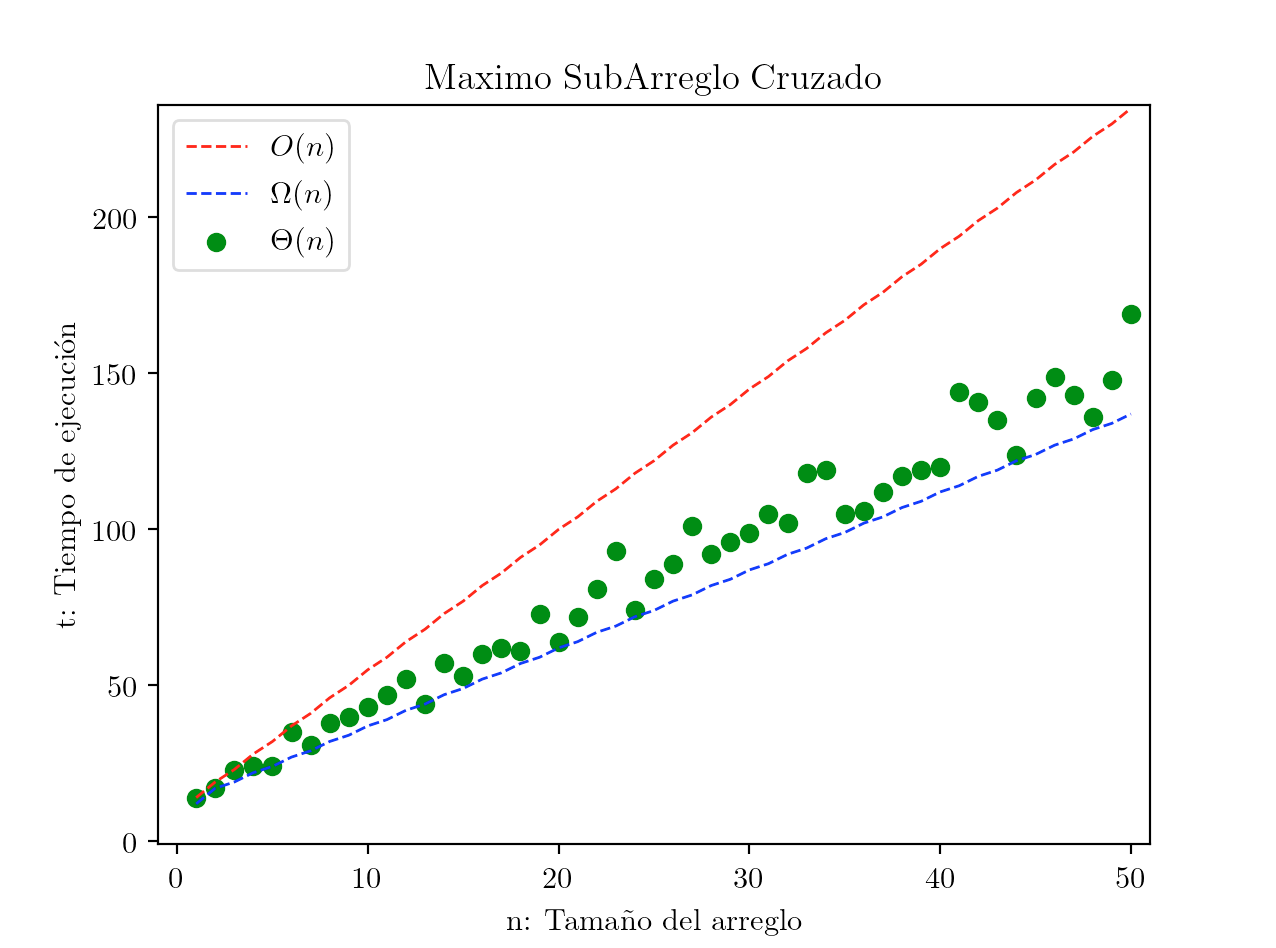
\includegraphics[height=0.75\textwidth]{Figure2}
  \caption{Máximo Subarreglo Cruzado}
  \label{fig:ejemplo1}
\end{figure}
\newpage

\subsection{\textbf{Máximo Subarreglo}}
\begin{algorithm}[h]
  \caption{Máximo Subarreglo}\label{euclid}
  \begin{algorithmic}[1]
  \Function{MS}{$A[0, ..., n-1], bajo, alto$}
    \If {$bajo = alto$}                                                              \Comment $O(1)$
      \State \textbf{return} $(bajo, alto, A[bajo])$                                 \Comment $O(1)$
    \Else
      \State $mitad \gets \lfloor \frac{bajo + alto}{2} \rfloor$                     \Comment $O(1)$
      \State $min\_izq, max\_izq, suma\_izq \gets MS(A,bajo,mitad)$                  \Comment $T(\frac{n}{2})$                                                
      \State $min\_der, max\_der, suma\_der \gets MS(A,mitad + 1,mitad)$             \Comment $T(\frac{n}{2})$  
      \State $min\_cruz, max\_cruz, suma\_cruz \gets MSC(A,bajo,mitad, alto)$        \Comment $O(n)$
      \If{$suma\_izq > suma\_der \&\& suma\_izq > suma\_cruz$}                       \Comment $O(1)$
        \State \textbf{return} $(min\_izq,max\_izq,suma\_izq)$                       \Comment $O(1)$
      \ElsIf{$suma\_der > suma\_izq \&\& suma\_der > suma\_cruz$}                 
        \State \textbf{return} $(min\_der,max\_der,suma\_der)$                       \Comment $O(1)$
      \Else                    
        \State \textbf{return} $(min\_cruz,max\_cruz,suma\_cruz)$                    \Comment $O(1)$
      \EndIf
    \EndIf
  \EndFunction
  \end{algorithmic}
\end{algorithm}
El algoritmo de \textbf{Máximo Subarreglo} podemos analizarlo de manera que ocurre una forma recursiva, por lo tanto haremos uso de un 
método que nos permita analizar este algoritmo recursivo, de lo cual haremos uso de \textbf{Recursividad de manera descendente}.

\begin{figure}[h]
  \centering
    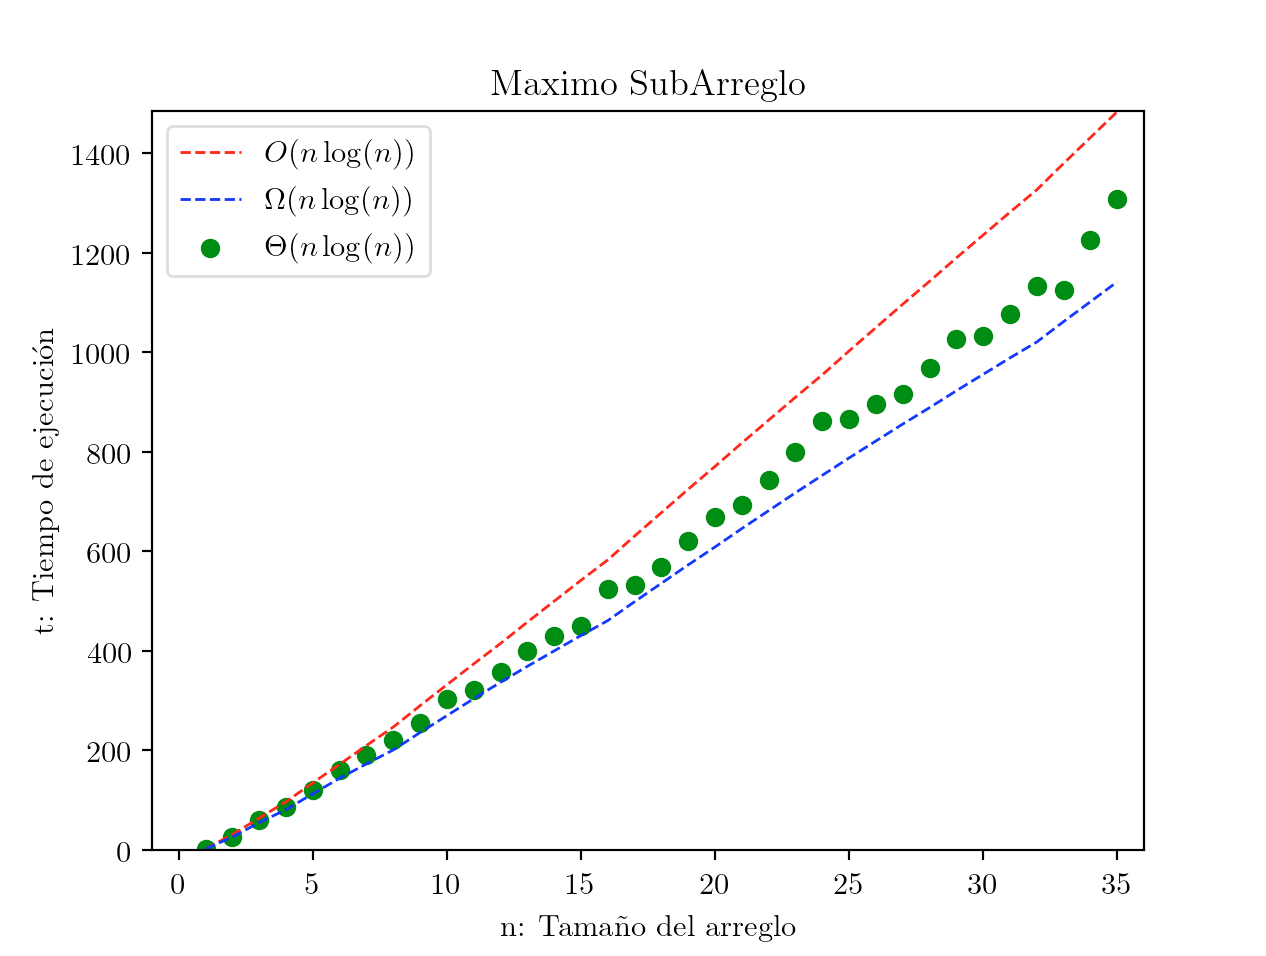
\includegraphics[height=0.75\textwidth]{Figure3}
  \caption{Máximo Subarreglo con Técnica Divide y Vencerás}
  \label{fig:ejemplo3}
\end{figure}

\centerline{}
\centerline{\textit{Se tiene la siguiente función de recursividad:}}
\begin{center}
  $T(n) =\left\{ \begin{array}{lcc}
      c_{1} &   si& n=1\\
  \\  2*T(\frac{n}{2}) + c_{2}*n + c_{3} &  si  & n>1 
  \end{array}
  \right.
  $
\end{center}

Debido a que no tenemos nocion acerca de $T(\frac{n}{2})$, optaremos por construir una nueva función de recurrencia a partir 
de la transformación $n = \log_{2} k \Rightarrow k = 2^n$. Entonces $T(n)$ en términos de $k$ sería:

\begin{center}
  $T(2^k) =\left\{ \begin{array}{lcc}
      c &   si& k=0\\
  \\  2*T(2^{k-1}) + c*2^k + c &  si  & k>0 
  \end{array}
  \right.
  $
\end{center}
\newpage

Se tiene:\\

  $T(2^k)=2*T(2^{k-1}) + c*2^k$\\
  $T(2^k)=2*[2*T(2^{k-2}) + c*2^{k-1}] + c*2^k$\\
  $T(2^k)=2^2*T(2^{k-2}) + 2*c*2^k$\\
  $T(2^k)=2^2*[2*T(2^{k-3}) + c*2^{k-2} + c] + 2*c*2^k$\\
  $T(2^k)=2^3*T(2^{k-3}) + 3*c*2^k$\\
  $\vdots$\\
  $T(2^k)=2^i*T(2^{k-i}) + i*c*2^k$\\ 
  \centerline{}
  Si $k = i$, entonces:\\
  $T(2^k)=2^k*T(1) + k*c*2^k$\\ 
  \centerline{}
  Regresando a $n$:\\
  $T(n)=n*T(1) + \log_{2}(n)*c*n$\\
  $\therefore T(n) \in O(n \log(n))$\\ \\

Con lo que podemos concluir que el algoritmo tiene una complejidad $O(n\log(n))$ y que se podría con siderar dentro de nuestras
opciones para aquellos problemas requeridos. Sin embargo aún queda por ver como es el comportamiento de éste mismo si lo intentamos
por fuerza bruta, ¿Mejorará?, ¿Empeorará?

\subsection{\textbf{Maximo Subarreglo por fuerza bruta}}
\begin{algorithm}[h]
  \caption{Máximo Subarreglo}\label{euclid}
  \begin{algorithmic}[1]
  \Function{MS}{$A[0, ..., n-1]$}                           
    \State $suma\_max \gets 0$                              \Comment $O(1)$
    \For{$i = 0$ \textbf{to} length of $A$}                 \Comment $O(n)$                      
      \State $suma \gets 0$                                 \Comment $O(1)$              
      \For {$j = i$ \textbf{to} length of $A$}              \Comment $O(n)$
        \State $suma \gets suma + A[j]$                     \Comment $O(1)$
        \If{$suma > suma\_max$}                             \Comment $O(1)$
          \State $suma\_max \gets suma$                     \Comment $O(1)$
        \EndIf
      \EndFor                                 
    \EndFor
    \State \textbf{return} $suma\_max$
  \EndFunction
  \end{algorithmic}
\end{algorithm}

El algoritmo de \textbf{Máximo subarreglo} por fuerza bruta, podemos analizarlo de tal manera que:

\centerline{$T(n) = O(1)+O(n)[O(1) + O(n)[3*O(1)]]$}
\centerline{}
\centerline{donde: $d = $ cantidad de digitos o letras de la entrada}
\centerline{}
\centerline{donde: $O(g(n))_{1} + O(g(n))_{2}+\cdots+O(g(n))_n = O(g(n))$}
\centerline{}
\centerline{$\Rightarrow T(n) = O(1)+O(n)[O(1) + O(n)[O(1)]]$}
\centerline{}
\centerline{$\Rightarrow T(n) = O(1) + O(n)*O(n)$}
\centerline{}
\centerline{donde: $O(f(n)) * O(g(n))= O(f(n)*g(n))$}
\centerline{}
\centerline{$\Rightarrow T(n) = O(1) + O(n^2)$}
\centerline{}
\centerline{donde: $O(f(n)) + O(g(n)) = O(h(n))$}
\centerline{y $h(n)$ es la funci\'on con mayor jeraqu\'ia respecto a $g(n)$ y $f(n)$}
\centerline{}
\centerline{$\therefore T(n) \in O(n^2)$}
\centerline{}
Donde podemos concluir que, de manera forzada nos crea una complejidad cuadrática($O(n^2)$), lo cual produciría un cambio radical en poder 
computacional exigiendo aún mas de lo que puede lograr una función de \textbf{Divide y Vencerás}, por lo que es conveniente aun hacer el manejo 
de la técnica que hacerlo por fuerza bruta. 
\begin{figure}[h]
  \centering
    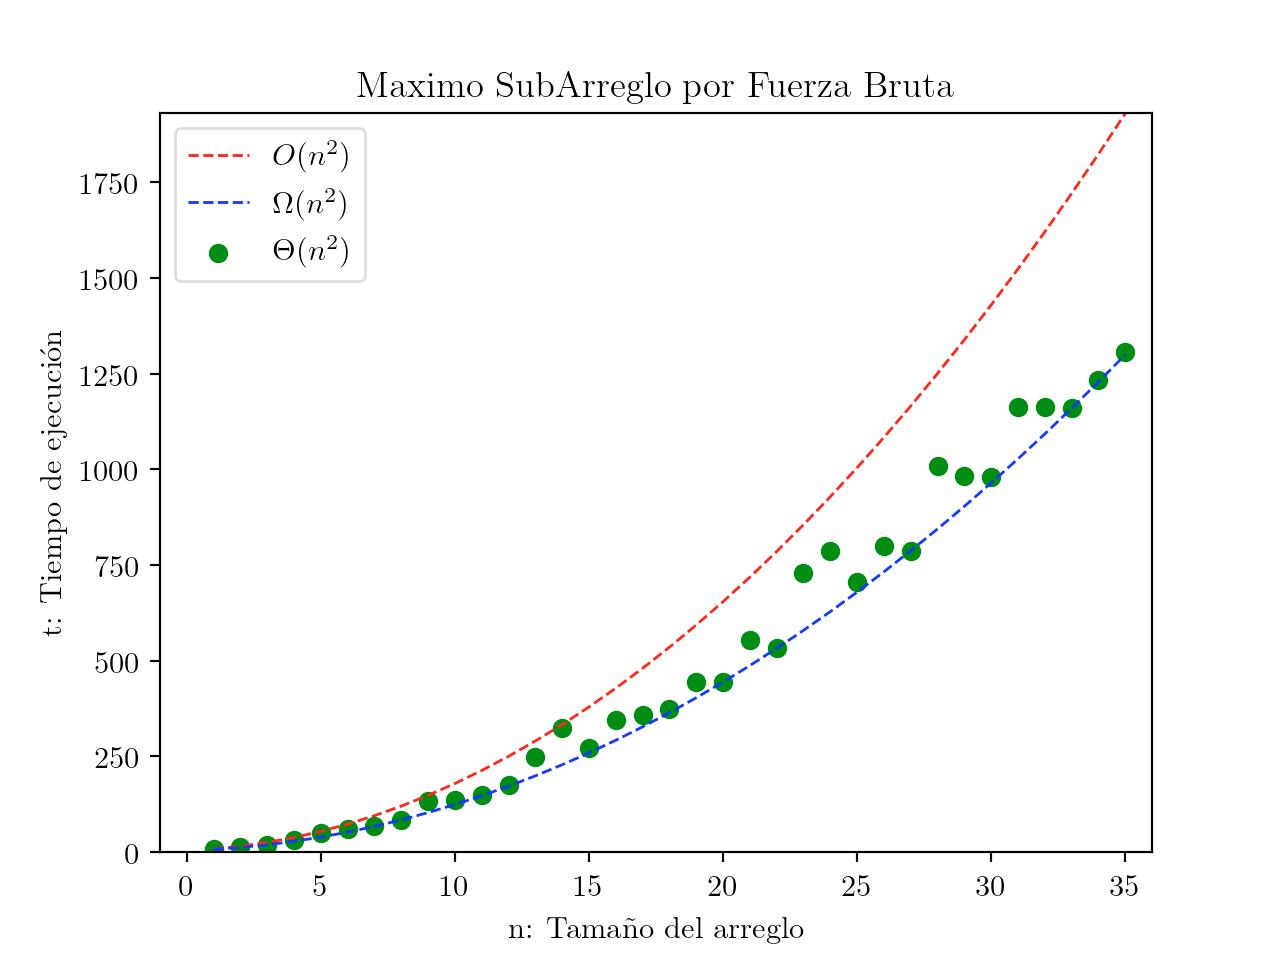
\includegraphics[height=0.75\textwidth]{Figure4}
  \caption{Máximo subarreglo por fuerza bruta}
  \label{fig:ejemplo3}
\end{figure}

\begin{figure}[h]
	\centering
	\begin{minipage}[t]{10cm}
		\centering
		
\includegraphics[scale=0.2]{Foto1}
		\caption{Alejandro Contreras Paredes}
	\end{minipage}
	\hspace{18cm}
	\begin{minipage}[t]{10cm}
		\centering
		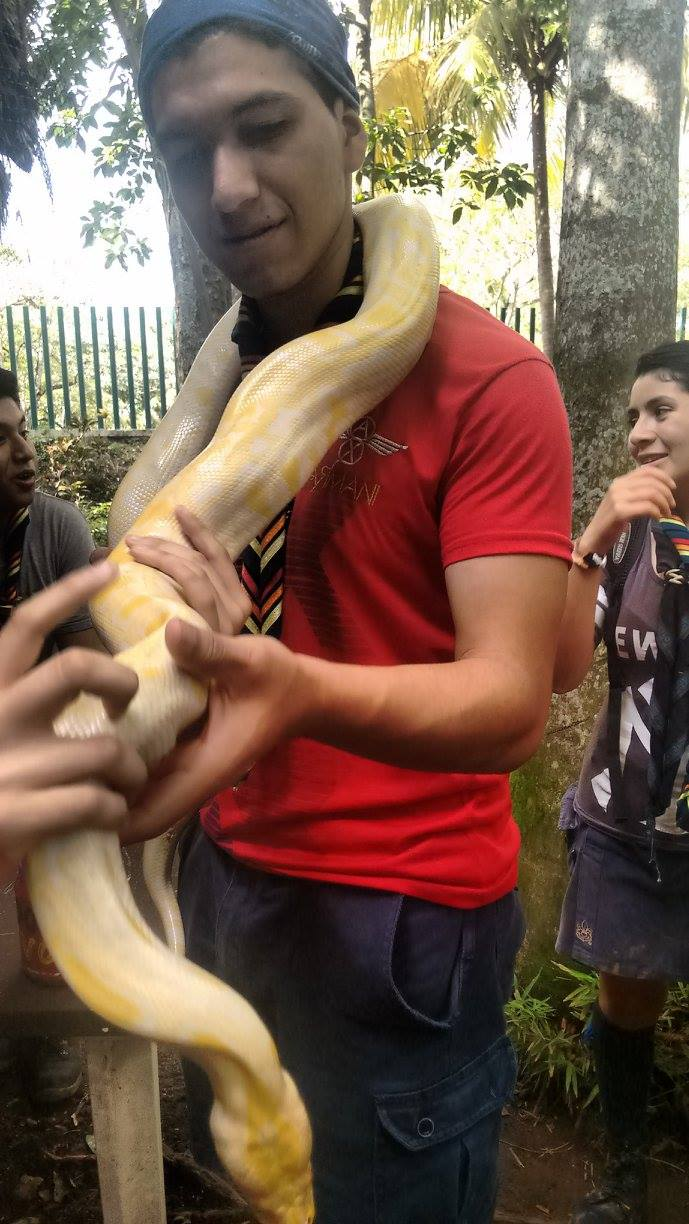
\includegraphics[scale=0.2]{Foto2}
		\caption{Rivera Paredes Fernando Daniel}
	\end{minipage}
\end{figure}
\newpage
\section{Anexo}
\centerline{\textbf{Preguntas}}

\textbf{1.-}\textit{¿Qué retorna la función de máximo subarreglo cuando todos los valores del arreglo son valores enteros negativos?}
\centerline{}
\textbf{R.} Depende del algoritmo deseado o utilizado, en tal caso, si hacemos uso del algoritmo por técnica de \textbf{Divide y Vencerás}
es evidente que el valor retornado de la suma mayor el numero negativo más cernano a cero, en conjunto con el índice máximo y mínimo
que aparentemente es el mismo. Ahora si hablamos del utilizado por fuerza bruta es evidente que ningun valor sería mayor que cero,
por lo que el valor de retorno sería cero.
\newpage
\section{Conclusiones}
\textbf{Conclusión Alejandro Contreras Paredes}\\
Está práctica resulta un poco confusa a mí manera de ver ya que la mera de plantear divide y vencerás es un poco diferente a lo que se a estado realizando en 
el pasado, al igual que otras ocasiones el quiso tuvo problemas con ciertos índices a la hora de la implementación, sin embargo se pudo solucionar de manera rapida. 
Por otro lado, el analizar la complejidad en el mejor o peor de los casos no resultó ser tan intuitiva y presentó una manera diferente de ver las cosas y aunque 
tomo su tiempo la práctica se pudo realizar sin problemas.\\\\
\textbf{Conclusión Fernando Daniel Rivera Paredes}\\
Comparar diferentes formas un algoritmo en específico ayuda a comparar los distintos puntos de vista a tomar en cuenta, no es sencillo realizar esa tarea, sin embargo
ya con la experiencia que uno va adquiriendo uno mismo. Al desarrollo de la misma qno interpreto gran desafio sn la parte de implementación, sin embargo, si hablamos
la lógica que ésta conlleva, determinar un peor y un mejor caso, analizar su comportamiento y determinar cuales serian los resultados de tal análisis antes de realizar
las pruebas, por lo que incrementa el tiempo brindado y da por entendido que es algo que hay q darle suficiente tiempo.

\section{Bibliograf\'ia}

\begin{thebibliography}{9}
  \bibitem{book} 
  Cormen, T. and Leiserson, C.
  \textit{Introduction to algorithms.} 
  3rd edition.Cambridge, Massachusetts: Massachusetts Institute of Technology, 2009.

  \bibitem{ie} 
  Moyano, N.
  \textit{Análisis de algoritmos}.
  Medium. Available at: $www.lcc.uma.es/~av/Libro/CAP3.pdf$'[Accessed 03 Sep. 2019].
\end{thebibliography}
\end{document}
